\documentclass[b5paper,11pt]{article}
\bibliographystyle{plain}

\usepackage{geometry}
\usepackage{amssymb,amsthm,bm,mathrsfs,mathtools}
\usepackage[usenames]{xcolor}
\usepackage{hyperref}
\usepackage{graphicx}
\graphicspath{{../"img/"}{../"figures/"}}

\usepackage{mycommands}
\newcommand{\numcircled}[1]{\raisebox{.5pt}{\textcircled{\raisebox{-.9pt} {#1}}}}
\newcommand{\Dmax}{\trdis_\mathsf{max}}
\newcommand{\InFmax}{\infid_\mathsf{max}}
\newcommand{\Psb}{\mathcal{P}_\mathrm{SB}}
\newcommand{\Odd}{\Omega_{\mathsf{DD}}}
\newcommand{\Opdd}{\Omega_{\mathsf{PDD}}}
\newcommand{\vOpdd}{\vec{\Omega}_{\mathsf{P}}}
\newcommand{\LO}[1]{\operatorname{LO}}
\newcommand{\alphat}{\widetilde{\alpha}}
\newcommand{\betat}{\widetilde{\beta}}

\newcommand{\Ppb}{\mathscr{P}_{\mathrm{0}}}
\newcommand{\Pcp}{\mathscr{P}_{\mathrm{c}}}
\newcommand{\wtP}{\widetilde{P}}
\newcommand{\wtH}{\widetilde{H}}
\newcommand{\wtO}{\widetilde{\Omega}}
\newcommand{\wtU}{\widetilde{U}}

\newcommand{\HB}{H_\mathrm{B}}
\newcommand{\HSB}{H_\mathrm{SB}}

\newcommand{\Heff}{H_\mathrm{eff}}
\newcommand{\HeffB}{H_\mathrm{eff,B}}
\newcommand{\HeffSB}{H_\mathrm{eff,SB}}

\newcommand{\ep}{\Phi_\mathrm{SB}}
\newcommand{\wtep}{\widetilde{\Phi}_\mathrm{SB}}
\newcommand{\epB}{\Phi_\mathrm{B}}
\newcommand{\phiB}{\phi_\mathrm{B}}

\newcommand{\CDDn}{\mathrm{CDD}_n}
\newcommand{\rDD}{\mathrm{DD}}
\newcommand{\rmax}{\mathrm{max}}
\begin{document}
\section{Note on noisy gates}
Previously, we treated the DD control gates in an ideal manner, which implies instantaneous and noise-free pulses. In practice, of course, the control gates are noisy quantum channels that need not be unitary.
Non-unitary channels are problematic for us as we can no longer use the error phase to characterize the noise strength.
However, one may always include an ancillary system to transform a quantum channel into a unitary one over the extended Hilbert space. For the analytical treatment below, we will always assume this dilation for the actual gates and marked the extended unitary operators with overtildes, e.g., $\wtP_i$. 
To facilitate our analysis, we ascribe Hermitian generators to the noisy gates. Such generator should be dominated by that of an ideal gate. In general, we should have 
\begin{equation}\label{eq:pulse-hami}
 \widetilde{P}_i= \exp\left[ -\upi \left( \Omega_{P_i} + \eta\, \Gamma_{P_i} \right)  \right],
\end{equation}
where $\Omega_{P_i}$ is responsible for the ideal $P_i$-gate and $\Gamma_{P_i}$ is a Hermitian generator responsible for the imperfection, $\eta$ is a small positive number for tracking the noise strength. While $\Omega_{P_i}$ is system-only, the noise part $\eta\Gamma_{P_i}$ is supported on the system-bath-ancilla composite in general. For Pauli group transformations in particular, we have $\Omega_{\sigma_i} = (\pi/2)\sigma_i$ generating a $\pi$-rotation.

A general DD sequence under those noisy pulses are then 
\begin{equation}\label{eq:noisy-UDD}
 \widetilde{U}_{\mathrm{DD}} =  \wtP_L \upe^{-\upi \Omega}  \ldots  \wtP_1\upe^{-\upi \Omega}\equiv  \upe^{-\upi\wtO_\rDD},
\end{equation}
where we also put tildes over $U_\rDD$ and $\Omega_\rDD$ to remind that the DD control gates are noisy. 
The overall goal is to figure out the conditions required by the noisy gates such that the noise-inflicted DD error phase $\wtep \equiv \norm{\wtO_{\rDD,\rSB}}$  is still reduced compared to the bare Hamiltonian error phase $\phi_\rSB = \norm{\Omega_{\rDD,\rSB}}$. For simplicity, let us employ a single parameter $\eta$, which is defined later,  to quantify the noise strength associated with the gates.  The break-even condition is, in essence, to invert the inequality
\begin{equation}
 \wtep(\phi_\rB,\phi_\rSB,\eta) < \phi_\rSB,
\end{equation} 
and obtain an upper bound on the noise level $\eta<\eta_{\rmax}(\phi_\rB, \phi_\rSB)$.
To achieve this, we need to correctly estimate the DD error phase function $\wtep(\phi_\rB,\phi_\rSB,\eta)$ while also looking for an appropriate definition for the noise strength $\eta$ associated with the gates.  

 A similar noise model was considered in Ref.~\!\cite{khodjasteh2007performance} for the case of finite-width pulses, where $ H'_{P_i} $ was set as $\delta H$ for all $\wtP_i$-gates (assuming the pulse duration $\delta$ and system-bath coupling Hamiltonian $H$). Our work improve upon the past work by allowing more generic type of noise while focusing on the break-even conditions for the DD sequence. 

One may now be tempted to plug \Eqref{eq:pulse-hami} into \Eqref{eq:noisy-UDD} to obtain the sequence unitary $\wtU_\rDD$ and solve for $\wtO_\rDD$. However, there is no way to directly derive a converging Magnus series for now as the convergence condition is violated by the very large $\norm{\Omega_{P_i}} >\xi$. Furthermore, we need Pauli operator conjugations for DD to function normally.  Therefore it is obligatory to separate out the ideal-gate part from the noisy gate.

\subsection{Gate-independent noise}
For each noisy gate $\wtP_i$, we may separate out a ``pure error'' map, $P_i^{\dagger} \wtP_i$, by applying the inverse gate.  As the resulting operator is unitary and close to identify,  we may associated to it a Hermitian generator $\Gamma_i$ to write the noisy gate as
\begin{equation}
 \wtP_i = P_i \upe^{-\upi \Gamma_i}.
\end{equation}
The evolution of the system and bath under noisy pulses thus becomes
\begin{equation}\label{eq:UDD-gatedep}
 \upe^{-\upi\wtO_\rDD} = P_L\upe^{-\upi \Gamma_L} \upe^{-\upi \Omega} \ldots  P_1\upe^{-\upi \Gamma_1}\upe^{-\upi \Omega }.
\end{equation}
The already established map $\Omega\to \Omega_{\rDD}$ for the idea-pulse DD sequence can no longer be reused, unless if the noise is gate-independent, i.e,
\begin{equation}\label{eq:gateindep1}
 \wtP_i = P_i \upe^{-\upi \Gamma},\ \forall i.
\end{equation}
Let us for now focus on such gate-independent noise. The problem readily reduces to the ideal DD case by replacing $\Omega=\tau H$ in our earlier analysis by $\wtO \equiv \tau \wtH$ such that
\begin{equation}
\upe^{-\upi \wtO}=\upe^{-\upi \Gamma}\upe^{-\upi \Omega}.
\end{equation}
Since $\Gamma$ and $\Omega$ are both small, as required for DD to work,
one may invoke the BCH formula to get $\wtO$ as a series of nested commutators. 
Similar to $\Omega=\Omega_\rB + \Omega_\rSB$, let us also split $\Gamma$ into the pure bath part $\Gamma_\rB$ plus the interaction part $\Gamma_\rSB$ and define 
$(\eta_0,\eta) \equiv (\Vert\Gamma_{\rB}\Vert, \Vert\Gamma_{\rSB}\Vert)$.
Assuming $\Gamma$ and $\Omega$ not particularly correlated, we may retain to the second order terms, and then apply triangular inequality to derive the upper bounds for $(\widetilde\phi_\rB,\widetilde{\phi}_\rSB) \equiv( \norm{\wtO_\rB}, \norm{\wtO_\rSB})$:
\begin{equation}\label{eq:comb-bound}
\left\{
\begin{aligned}
 \widetilde\phi_\rB &\lesssim (\eta_0 + \phi_\rB)(1+\eta + \phi_\rSB) \equiv \widetilde\phi_\rB^{(\mathrm{ub})}\\
 \widetilde\phi_\rSB &\lesssim (\eta + \phi_\rSB) (1+\eta_0 + \phi_\rB)\equiv \widetilde\phi_\rSB^{(\mathrm{ub})}
\end{aligned}
\right..
\end{equation}
In Fig.~\ref{fig:approx-bound}, we numerically verify this approximate bounds by randomly generating small $\Gamma$ and $\Omega$ operators and compute $(\widetilde\phi_\rB,\widetilde{\phi}_\rSB)$ for the combined $\wtO$.
The result seems positive with no violation found.
With this, we can bound the error phase relevant for this noisy-pulse situation under the different schemes by replacing $\phi_\rB$ and $\phi_\rSB$ for the ideal case with their noisy upper bounds: 
\begin{equation}
 \widetilde\Phi_\rSB \le \Phi_\rSB(\widetilde\phi_\rB^{(\mathrm{ub})}  ,\widetilde\phi_\rSB^{(\mathrm{ub})} ) < \phi_\rSB.
\end{equation}
Further bounding the right hand side by $\phi_\rSB$ then gives us the condition for the break-even points.

\begin{figure}[htbp]
 \centering
 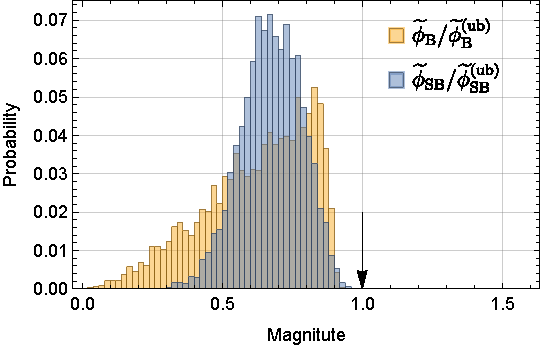
\includegraphics[width=0.8\linewidth]{approx-bound}
 \caption{The histogram for $\widetilde\phi_\rB/\widetilde\phi_\rB^{(\mathrm{ub})}$ and $\widetilde\phi_\rSB/\widetilde\phi_\rSB^{(\mathrm{ub})}$ over 5000 randomly generated $\Gamma$ and $\Omega$ ($2\times2$) matrices. The random $\Gamma$ and $\Omega$ are set to be have the magnitudes around $0.01$ under a normal distribution. Our appropriate bounds in \Eqref{eq:comb-bound} is indicated with an arrow.}
 \label{fig:approx-bound}
\end{figure}


The above analysis is generic and applies to all DD schemes with gate-independent noise. 
The resulting bound is general, but could be suboptimal for a specific DD scheme and a specific type of pulse imperfection. Below, we examine a concrete examples of imperfections  for PDD: 
global unitary error in the control gates,  which results in the noisy pulse 
\begin{equation}
\widetilde P_i=P_i\upe^{-\upi \bm{\theta}\cdot\bm\sigma},\ \forall i.
\end{equation}
We use the notation $\bm\sigma\equiv (X,Y,Z)=(\sigma_1,\sigma_2,\sigma_3)$, and $\bm\theta\equiv (\theta_1,\theta_2,\theta_3)$ with $\theta_i$ real constants---taken as small for weak noise---that parameterize the unitary error.  This can arise from, for example, a systematic calibration error in the pulse control leading to a consistent over or under rotation. \rsout{One could also include in this model a random over/under-rotation by drawing $\theta$ from a specified distribution that describes the randomness in the control. Here, we restrict to the systematic error case and note only that our analysis applies to this random error situation simply by doing an average over the distribution of $\bm\theta$.} \gray{(Random unitary rotation does not fit into the gate-independent noise model. So it is not suitable for discussion here.)}
\rsout{For simplicity, we assume gate-independent noise, so the same $\bm\theta$ applies to all pulses. } In this situation, $\Gamma\equiv \bm\theta\cdot\bm\sigma$ acts only on the system. 

We can write the effective noisy Hamilton operator as
\begin{equation}
\widetilde H\equiv \bm\theta\cdot\bm\sigma+H',
\end{equation}
where $H'\equiv \sum_{i=1,2,3}\sigma_i\otimes B_i'$s, with $B_i'$ to be related to the $B_i$s in the original $H$. Keeping up to the second-order term in the BCH series of Eq.~\eqref{eq:BCH_Htilde}, straightforward algebra yields $B_0'\simeq B_0$, and $B_i'\simeq B_i+\sum_{jk=1,2,3}\epsilon_{ijk}\theta_j B_k$, for $i=1,2,3$, and $\epsilon_{ijk}$ is the completely anti-symmetric tensor.
To lowest order in $\vec\theta$, we can regard $(B_1',B_2',B_3')$ as a rotation of $(B_1,B_2,B_3)$ with respect to the $\vec\theta$-axis. 
\blue{(To check this and merge with the new text.)} \gray{On the other hand,  we know from its definition that the error phase is the invariant with respect to a basis change of the system, which acts as a 3D rotation on the vector $(B_1,B_2,B_3)$.
As a result, the error phase of $\Omega'$ remains identical to $\beta$ up to the second order in $\theta$.}

\gray{To conclude, the two-component norm of $\Omega'$ can be estimate by
\begin{equation}\label{eq:eff-Hami-tcp}
    \opnorm{\Omega'} = \begin{pmatrix}
        \alphat \\
        \beta'
    \end{pmatrix}
    \le 
    \begin{pmatrix}
        \alpha + \frac{1}{3}\theta\beta^2  \\
        \beta + \theta^2 \beta
    \end{pmatrix}.
\end{equation}
Assuming the noise to be small, we may only use the leading order 
approximation, knowing that it is accurate to the second order. 
}
\red{Where do the $\widetilde\alpha$ and $\beta'$ expressions come from? I see that the $\widetilde\alpha$ one comes from setting $\Gamma_\mathrm{SA}=\tau\vec\theta\cdot\vec\sigma$ and hence $\eta\equiv\tau\Vert\Gamma_{\mathrm{SA}}\Vert\propto \theta$, and then plugging that into Eq. (69) of the earlier draft, with $\eta_0=0$. But why is the proportionality constant $1$? What is the norm used here?
Same question for $\beta'$: Where does the coefficient for the $\theta^2\beta$ come from? I'm understanding that we don't have a linear-in-$\theta$ term because of the rotation argument above, but that does not explain the coefficient of 1 for the quadratic term. Is it just a matter of algebra using the BCH formula for the next-order terms?

Also, how is $\theta$ related to the vector $\vec \theta$? What norm is being used for this?
}

\noindent\blue{(I'm holding off on editing the rest of this section until I get better clarity on the above questions. Retain only the PDD discussion here; CDD discussion goes into the next section. Also need to put back the argument leading up to Eq.~(69) of the earlier draft for when $\Gamma$ acts purely on the system and not on the bath.) }



\subsection{Gate-dependent noise}
For the more generic case of gate-depend noise,  we can no longer reuse the ideal DD transformation formula $\Omega\to\Omega_\rDD$ as there is no 
well defined $\Omega$. But we can still rewrite \Eqref{eq:UDD-gatedep} to allow derivation of a converging series for $\Omega_\rDD$:
\begin{equation}
\begin{aligned}
  \upe^{-\upi\wtO_\rDD} = \upe^{-\upi  G_L \Gamma_L  G_L^\dagger} \upe^{-\upi \Omega_L}   \ldots \upe^{-\upi  G_2 \Gamma_2  G_2^\dagger} \upe^{-\upi \Omega_2}  \upe^{-\upi \Gamma_1}\upe^{-\upi \Omega_1}.
\end{aligned}
\end{equation}
As all the matrix exponents are small, we may use the Magnus formula to derive the leading order Magnus series as good approximation to $\wtO_\rDD$.

For concreteness, let's consider PDD, where the sequence comprises only $X$ and $Z$ gates. This amounts to writing the noisy $X$ and $Z$ pulses as
\begin{equation}\label{eq:gatedep-noise}
\widetilde{X} = X \upe^{-\upi \Gamma'}\quad\textrm{and}\quad \widetilde{Z} = Z \upe^{-\upi \Gamma''}.
\end{equation}
Here, $\Gamma'$ and $\Gamma''$ can generally act on the system and bath (including possibly an ancillary system). 
We define
\begin{equation}
\Gamma' \equiv \sum_i \sigma_i \otimes B'_i \quad \text{and} \quad
\Gamma'' \equiv \sum_i \sigma_i \otimes B''_i.
\end{equation}
The time evolution over the noisy PDD sequence then becomes
\begin{align}
\upe^{-\upi \widetilde\Omega_\mathrm{PDD} } =
 \upe^{-\upi Z \Gamma'' Z} \upe^{-\upi \Omega_3}
 \upe^{-\upi Y \Gamma' Y} \upe^{-\upi \Omega_2}
  \upe^{-\upi X \Gamma'' X} \upe^{-\upi \Omega_1}
    \upe^{-\upi \Gamma'} \upe^{-\upi \Omega}.
\end{align}
Every term on the exponent is now small and we can apply the Magnus formula to evaluate $\widetilde\Omega_\mathrm{PDD}$.
For the first order term: 
\begin{equation}\label{eq:PDD-gatedep-Mag1}
\begin{aligned}
 \widetilde{\Omega}_\mathrm{PDD}^{(1)} 
&= \sigma_0 \otimes (4B_0 + 2 B'_0 + 2B''_0) \\
&+ \sigma_2 \otimes (2B_2'-2B_2'').
\end{aligned}
\end{equation}
When the noise is gate-independent, i.e., when $\Gamma'=\Gamma''$, the expression reduce back to the ideal PDD situation, consistent with our earlier discussion for the gate-independent imperfections. 
With gate-dependent noise, however, exact first order decoupling is lost, as the coupling part  no longer vanishes in the first order Magnus term. 
This has significant implication for the concatenate DD scheme as well, 
as the first order coupling would persist throughout all concatenation levels. 

The term that acts nontrivially on the system in $\widetilde \Omega_\mathrm{PDD}^{(1)}$ is proportional to $B_2'-B_2''$. Analogous to the gate-independent noise situation, we take $\eta\equiv \max\{\Vert \Gamma_X\Vert,\Vert \Gamma_Z\Vert\}$. Assuming no particular relation between the $X$ and $Z$ noise,  we upper-bound the size of the first order coupling by:
\begin{equation}\label{eq:gatedep-upperbound}
\norm{ \widetilde{\Omega}_\mathrm{PDD:SB}^{(1)} } \le 4 \eta.
\end{equation}
When the gate noise is at least of similar strength as the noise from $H_\mathrm{SB}$---the gate noise is in fact stronger than the background noise in many experiments---$\widetilde{\Omega}_\mathrm{PDD}$ is dominated by the first order term. So that the error phase for PDD can be estimated as $\ep\simeq \norm{ \widetilde{\Omega}_\mathrm{PDD:SB}^{(1)} } \leq 4\eta$.
With this estimate, the condition for the break-even point for PDD under such gate-dependent noise can be written as 
\begin{equation}
4\eta\leq\phi_\rSB.
\end{equation}

 \begin{figure}
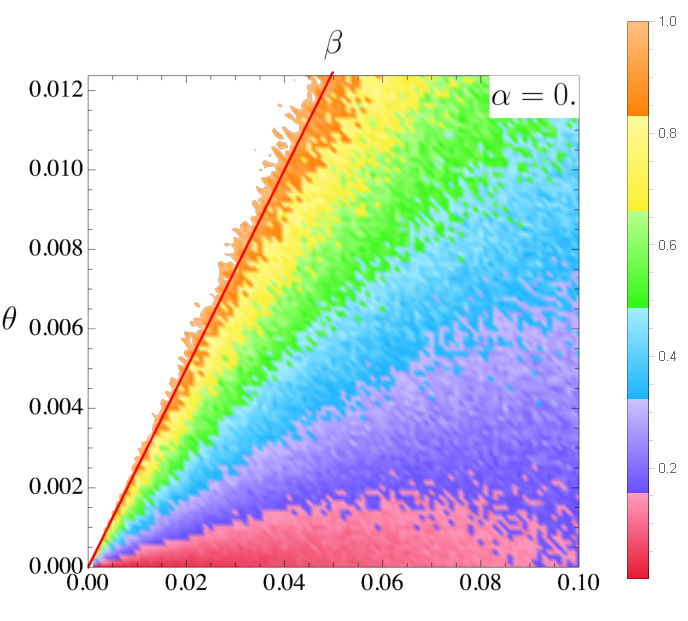
\includegraphics[width=0.45\linewidth]{pdd-gatedep-thres}\quad
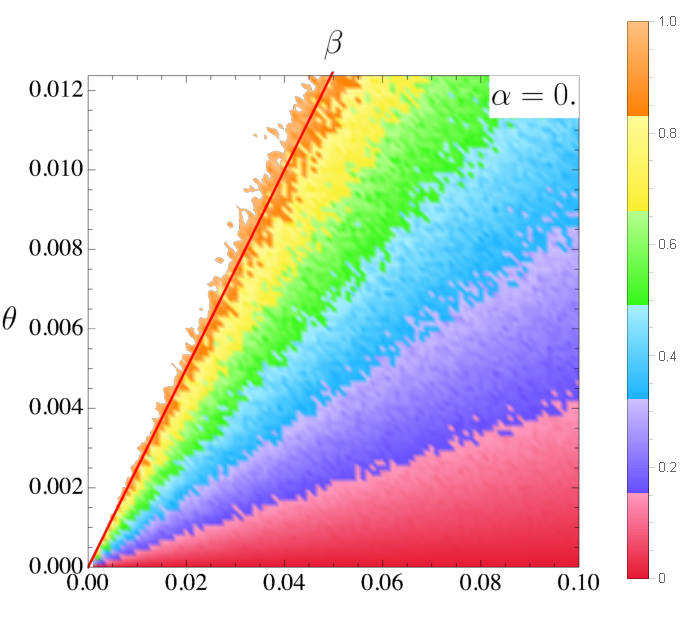
\includegraphics[width=0.45\linewidth]{cdd-gatedep-thres}
\caption{\red{(Which one is for PDD? Why do some points violate the threshold condition? Is it because of numerical---sampling?---inaccuracies?) }The noise threshold compared for PDD and $\mathrm{CDD}_3$ simulated at $\alpha=0$. The red solid line represents the noise threshold prediction $\eta\le\beta/4$. different colors represents different levels of noise reduction ration $\beta_\sDD/\beta$ after numerically maximized over random bath operator instances.
\label{fig:cdd-gatedep-thres}}
\end{figure}

\red{(Please provide more details for the figure, on how the numerics are done. For example, what random bath operators are we referring to? The $B'$s and $B''$s? What do you mean by ``random" here? Uniform distribution over what? Initial system and bath states? etc.) }\gray{In \Figref{fig:cdd-gatedep-thres}, we simulate both PDD and $\mathrm{CDD}_3$ with the gate-dependent noise model. We find that our prediction works pretty well. 
}





\subsection{Gate-independence version 2}
The decomposition $\wtP_i = P_i \upe^{-\upi \Gamma_i}$  previously considered for the noisy gate is by construction and not fundamental. 
Another possible decomposition is to include both left-error and right-error maps, as opposed to only one-sided error map. That is,
\begin{equation}\label{eq:leftright-noise}
 \wtP_i = \upe^{-\upi L_i} P_i \upe^{-\upi R_i},
\end{equation}
where $L_i$ and $R_i$ are gate-dependent Hermitian operators responsible for generating the left and right error maps.  We expect both operators  to be small as the noise is weak.
Using this decomposition, we get another definition for gate-independent noise. We say that the noise associated with the gate is gate-independent if there exists Hermitian $L$ and $R$ operators such that 
$L_i=L$ and $R_i = R$ for all noisy pulses $\wtP_i$. This definition automatically cover the previous one by setting $L_i=0$.
After plugging the gate-independent noise model into the DD sequence, one finds that 
\begin{equation}\label{eq:gateindep}
 \upe^{-\upi\wtO_\rDD} = \upe^{-\upi L} \left( P_L \upe^{-\upi \wtO} \ldots  P_1 \upe^{-\upi \wtO } \right) \upe^{\upi L},
\end{equation}
where we have defined the effective free-evolution Hamiltonian $\wtO$ by 
\begin{equation}
 \upe^{-\upi \wtO} = \upe^{-\upi R}  \upe^{-\upi \Omega}  \upe^{-\upi L}.
\end{equation}
In the bracket of \Eqref{eq:gateindep}, the sequence once again reduces to that of ideal DD gates. Therefore, the decoupling order will be unaffected within the bracket. The edge terms  $\upe^{\pm \upi L}$ in \Eqref{eq:gateindep}  seems to be problematic, as they will break the exact decoupling enjoyed by previously considered gate-independent noise. 
In fact, one need not be worried about the edge terms if DD is periodically performed in a long run. This is commonly assumed for both quantum memory and quantum computation tasks. Within the typical decoherence time for a NISQ era qubit, thousands of gates, if not more, can be performed. Naturally, a DD-protected task will involve in way more than one DD cycle. 
After joining these cycles, the edge terms will travel to the edges of the whole sequence, where they are usually overwhelmed by the state preparation and measurement errors. 
We do acknowledge these potential slight overheads, but the scaling benefit provided by DD are more meaningful. Hence it is safe to ignore these edge terms. 

A gate-independent noise with both left and right errors may may be viewed as gate-dependent in if only right noise is considered. This difference is only a superficial matter on the definitions. But how about the decoupling behavior? 
From previous discussion we know that gate-dependent noise will result in inexact decoupling, but gate-independent noise will have exact decoupling similar to the ideal case. To investigate this contraction, we consider PDD as an example. After equating both ways of decomposing the noisy gate, we have:
\begin{equation}
 \begin{split}
  \upe^{-\upi L} X \upe^{-\upi R} &=  X \upe^{-\upi \Gamma'},\\
  \upe^{-\upi L} Z\upe^{-\upi R} &=  Z \upe^{-\upi \Gamma''}.
 \end{split}
\end{equation}
For given $L$ and $R$, we can solve for $\Gamma'$ and $\Gamma''$ by basic algebra and the BCH formula. But the reverse is generally unsolvable. Since both $L$ and $R$ are small, we may truncate to the second order expansion:
\begin{equation}
 \begin{aligned}
  \Gamma' &= XLX +R + \frac{1}{2\upi} [XLX, R ] + \cdots, \\
   \Gamma'' &= ZLZ +R + \frac{1}{2\upi} [ZLZ, R ] + \cdots. 
 \end{aligned}
\end{equation}
According to \Eqref{eq:PDD-gatedep-Mag1}, the DD effective Hamiltonian has a non-vanishing  first order  coupling, which is proportional to $B_2'-B_2''$. 
Let us introduce a smallness parameter $\eta$ by shifting $L\to \eta L$ and $R\to \eta R$. We can use the formula for $\Gamma'$ and $\Gamma''$ to show that 
\begin{equation}
 B_2'-B_2''=\cO(\eta^2).
\end{equation}
Hence one can still argue that the first order decoupling is exact despite it is superficially not so. Exact decoupling or not is only a matter of perspective. We say PDD achieves first order decoupling because the first order smallness in the effective Hamiltonian is removed. This settles the decoupling order disagreement between the two views of gate-independence. 

How useful is the gate-independent noise model anyway? One may scorn it off as being too contrived and does not bear any practical relevance. To counter this doubt we consider the finite-width pulse noise model from a new perspective. The noisy gates are approximately:
\begin{equation}
 \upe^{-\upi (\frac{\pi}{2}\sigma_\alpha + \delta H)} \approx \upe^{-\upi  \frac{1}{2}\delta H} \upe^{-\upi \frac{\pi}{2}\sigma_\alpha} \upe^{-\upi  \frac{1}{2}\delta H}, \quad\text{for }\alpha=X,Z.
\end{equation}
This is an example of the Trotter-Suzuki type of approximation. And 
our approximation is valid to the second order as one may check. For PDD and CDD, all we will be concerned is the first two orders of Magnus term. Hence it suffices to use this approximation.

We now make the above observation rigorous. 

Proposition 1: For PDD if the Hermitian generator responsible for the noise is gate-independent. We have exact first order decoupling. 

Proposition 2: For CDDn if the Hermitian generator responsible for the noise is gate-independent. We have exact n-th order decoupling. 

\subsection{Unitary control noise with finite-width pulses}
\bibliography{references}
\end{document}